\documentclass[11pt]{article}
\usepackage[margin=1in]{geometry}
\usepackage[utf8]{inputenc}
\usepackage[T1]{fontenc}
\usepackage{booktabs,graphicx,amsmath,amssymb,hyperref,natbib}
\graphicspath{{figures/}}
\title{When Does a Cheap-First Cascade Keep Its Promise?\\
\large Threshold Selection with Statistical Guarantees: A Small-Scale Empirical Study}
\author{Arpit Pandey}
\date{DRAFT --- not for distribution; numbers are generated from \texttt{results/} and may change}
\begin{document}
\maketitle

\begin{abstract}
Systems that replace repeated LLM classification calls with a cheap student model behind a
confidence gate must choose a threshold. A common choice is the most lenient threshold whose
empirical agreement with the LLM on a calibration sample meets a target. We study how often such
selection violates its target, what it costs to replace it with selection that carries a
finite-sample guarantee, and what changes when the reference is a real, imperfect LLM and when
traffic drifts. Using frozen sentence embeddings with a logistic-regression student on Banking77
and CLINC150, we find that naive selection misses its target in roughly half of calibration draws,
by small margins; Bonferroni- and Holm-corrected Clopper--Pearson selection keeps violations far
below the nominal level at a cost of roughly four to twelve points of coverage at 1{,}000--2{,}000
audited examples. With a real teacher (Claude Haiku 5.5; 76.5\% and 90.9\% agreement with gold
labels), the guarantees still hold for the teacher-agreement target, but agreement is neither
sufficient nor necessary for correctness: a student distilled from the teacher violated a
gold-error target in 70\% of draws on Banking77, while a gold-trained student exceeded the teacher's
accuracy and was under-deployed by the agreement gate. In synthetic drift streams built from real
embeddings, rolling recalibration on uniformly audited labels reduced violations under mild shifts
but not under severe ones, and an anytime-valid monitor avoided the false alarms of a repeatedly
evaluated z-test at the price of delay. All results are small-scale (one encoder, one student
family, few splits) and preliminary.
\end{abstract}

\section{Introduction}
Describe the deployment setting (repeated closed-set LLM decisions), the cheap-first cascade, and
the threshold-selection question. Credit TRACER~\cite{rida2026tracer} precisely: it already
implements trace-trained students behind an agreement gate and a one-shot final certification.
State the contribution narrowly: an empirical comparison of selection procedures and a documented
pitfall, not the cascade idea.

\section{Related work}
LLM cascades and routing~\cite{chen2023frugalgpt,gupta2024cascades}; conformal and
distribution-free abstention~\cite{yadkori2024conformalabstention,angelopoulos2021gentle};
risk control by testing~\cite{angelopoulos2021ltt};
selective classification with a guaranteed risk, which already selects a confidence threshold with
a binomial bound and a Bonferroni correction~\cite{geifman2017selective};
cascades with distribution-free guarantees~\cite{conformalcascade2026,balancerag2026};
anytime-valid monitoring~\cite{waudbysmith2020betting,podkopaev2021tracking}; multiple testing~\cite{holm1979}; exact
binomial intervals~\cite{clopper1934}; TRACER~\cite{rida2026tracer}. Our Bonferroni and Holm
selection over a fixed grid is an application of this line of work (in particular the
selective-classification algorithm of Geifman and El-Yaniv) and is not claimed as new; see
\texttt{docs/notes/literature-check.md}.

\section{Setting and selection procedures}
Define score $c(x)$, error indicator $e$, risk $R(t)=P(e=1\mid c\ge t)$, coverage, target
$\alpha$, confidence $\delta$. Describe the compared procedures: naive, safety factor, Wilson
(uncorrected), certify-once, strict-start fixed sequence, Bonferroni over a fixed grid, Holm
step-down, split sequence. State the validity argument for each valid procedure and its
assumptions (i.i.d.\ calibration data; a grid fixed before seeing data).

\section{Experiments}
Datasets~\cite{casanueva2020banking77,larson2019clinc150}, embeddings, student, finite-population
protocol, number of splits and draws. All figures and tables are generated by
\texttt{scripts/make\_figures.py} from \texttt{results/}.

\begin{figure}[t]\centering
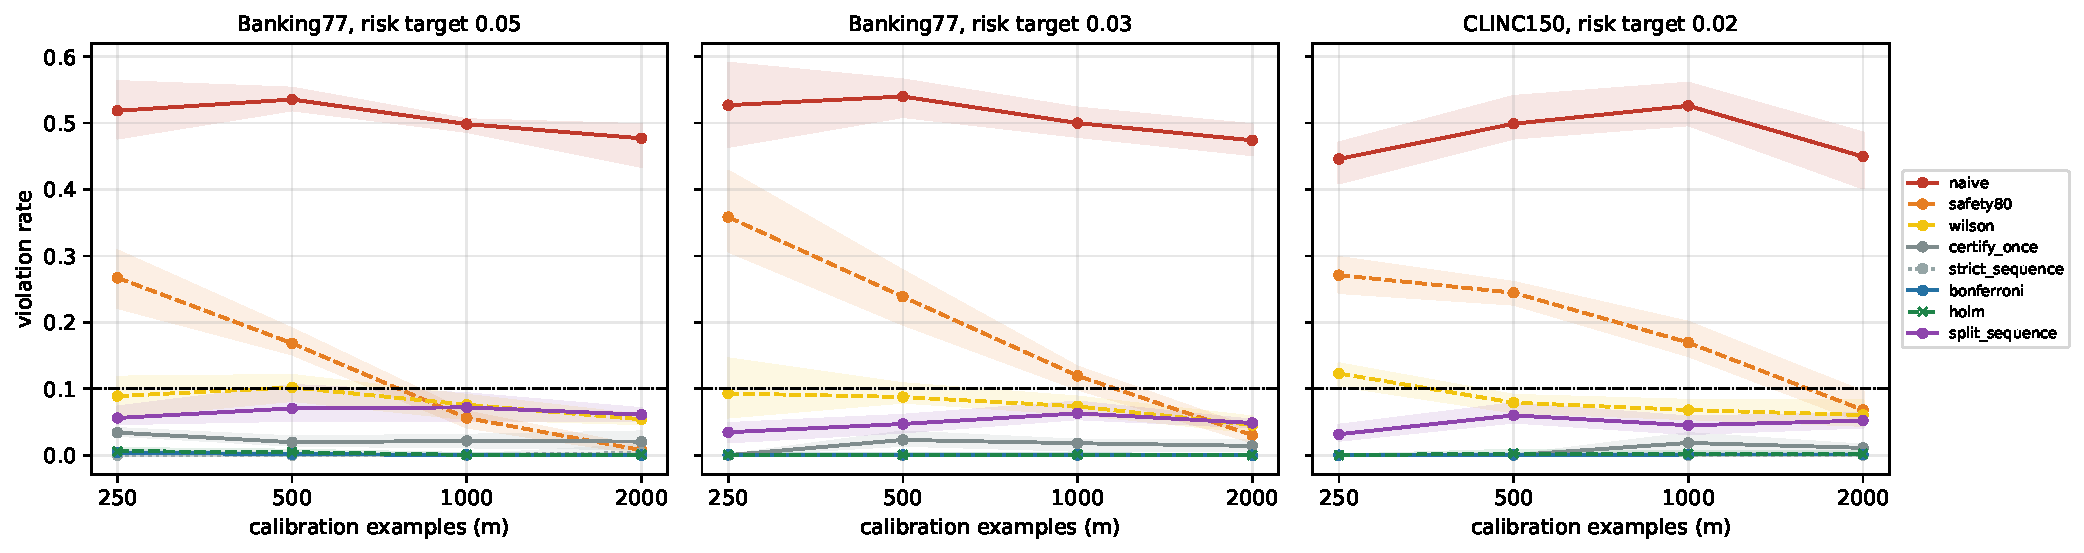
\includegraphics[width=\textwidth]{fig1_violation_vs_m.pdf}
\caption{Violation rate versus calibration size (dashed-dotted line: $\delta=0.10$). Bands show
min--max across splits.}\end{figure}

\begin{figure}[t]\centering
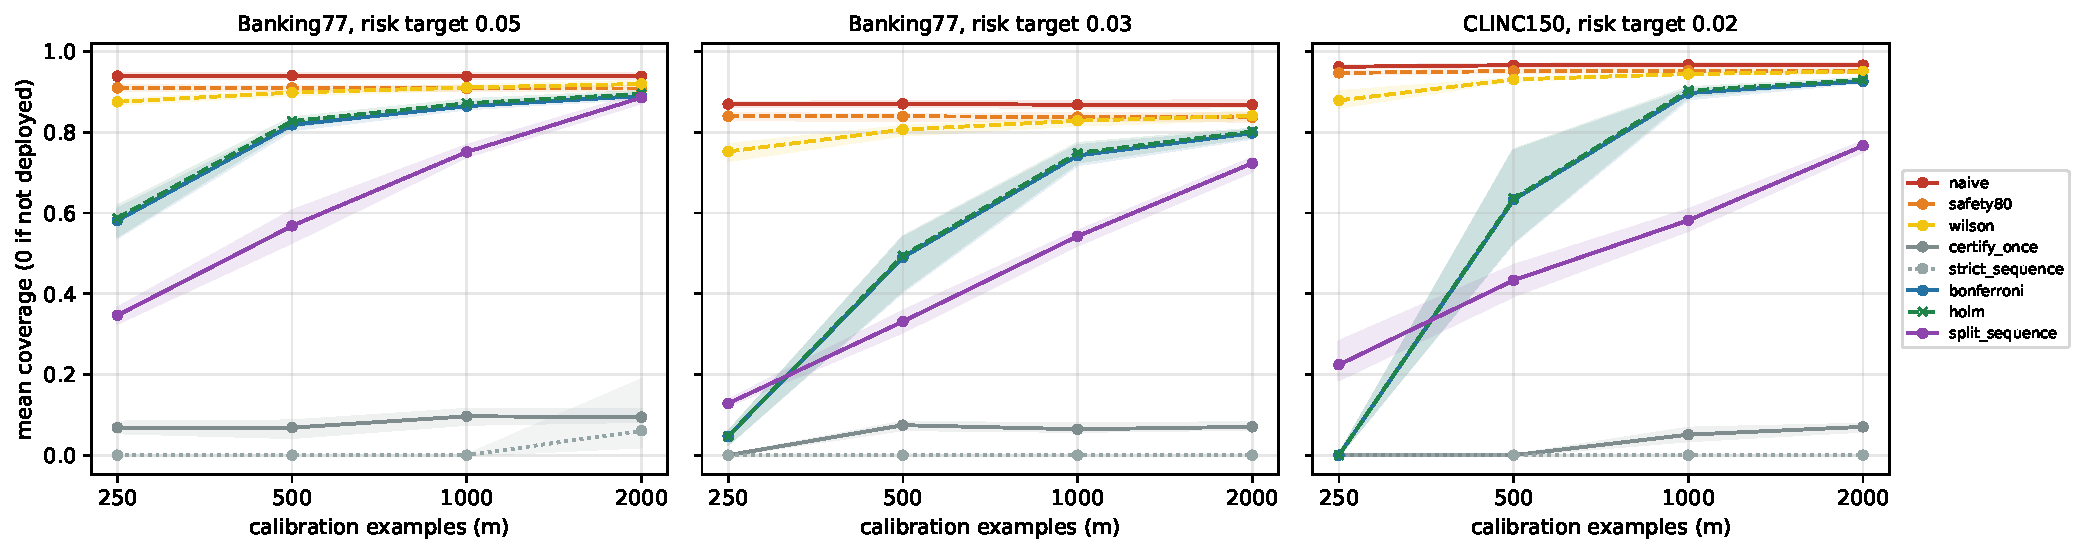
\includegraphics[width=\textwidth]{fig2_coverage_vs_m.pdf}
\caption{Mean coverage versus calibration size (0 when no threshold is deployed).}\end{figure}

\begin{table}[t]\centering\footnotesize
\begin{tabular}{llrlrrr}
\toprule
Task & $\alpha$ & $m$ & Method & Violation & Coverage & Deploy \\
\midrule
Banking77 & 0.05 & 1000 & naive & 0.499 & 0.939 & 1.00 \\
Banking77 & 0.05 & 1000 & wilson & 0.076 & 0.911 & 1.00 \\
Banking77 & 0.05 & 1000 & bonferroni & 0.001 & 0.865 & 1.00 \\
Banking77 & 0.05 & 1000 & holm & 0.001 & 0.872 & 1.00 \\
Banking77 & 0.05 & 2000 & naive & 0.477 & 0.939 & 1.00 \\
Banking77 & 0.05 & 2000 & wilson & 0.054 & 0.920 & 1.00 \\
Banking77 & 0.05 & 2000 & bonferroni & 0.000 & 0.890 & 1.00 \\
Banking77 & 0.05 & 2000 & holm & 0.001 & 0.895 & 1.00 \\
Banking77 & 0.03 & 1000 & naive & 0.500 & 0.868 & 1.00 \\
Banking77 & 0.03 & 1000 & wilson & 0.074 & 0.829 & 1.00 \\
Banking77 & 0.03 & 1000 & bonferroni & 0.001 & 0.742 & 1.00 \\
Banking77 & 0.03 & 1000 & holm & 0.001 & 0.749 & 1.00 \\
Banking77 & 0.03 & 2000 & naive & 0.474 & 0.868 & 1.00 \\
Banking77 & 0.03 & 2000 & wilson & 0.045 & 0.841 & 1.00 \\
Banking77 & 0.03 & 2000 & bonferroni & 0.000 & 0.798 & 1.00 \\
Banking77 & 0.03 & 2000 & holm & 0.000 & 0.802 & 1.00 \\
CLINC150 & 0.02 & 1000 & naive & 0.526 & 0.967 & 1.00 \\
CLINC150 & 0.02 & 1000 & wilson & 0.068 & 0.944 & 1.00 \\
CLINC150 & 0.02 & 1000 & bonferroni & 0.001 & 0.897 & 1.00 \\
CLINC150 & 0.02 & 1000 & holm & 0.002 & 0.903 & 1.00 \\
CLINC150 & 0.02 & 2000 & naive & 0.450 & 0.966 & 1.00 \\
CLINC150 & 0.02 & 2000 & wilson & 0.060 & 0.951 & 1.00 \\
CLINC150 & 0.02 & 2000 & bonferroni & 0.001 & 0.926 & 1.00 \\
CLINC150 & 0.02 & 2000 & holm & 0.002 & 0.930 & 1.00 \\
\bottomrule
\end{tabular}

\caption{Headline cells (generated from \texttt{results/}); all gates are in \texttt{results/SUMMARY.md}.}\end{table}

\begin{figure}[t]\centering
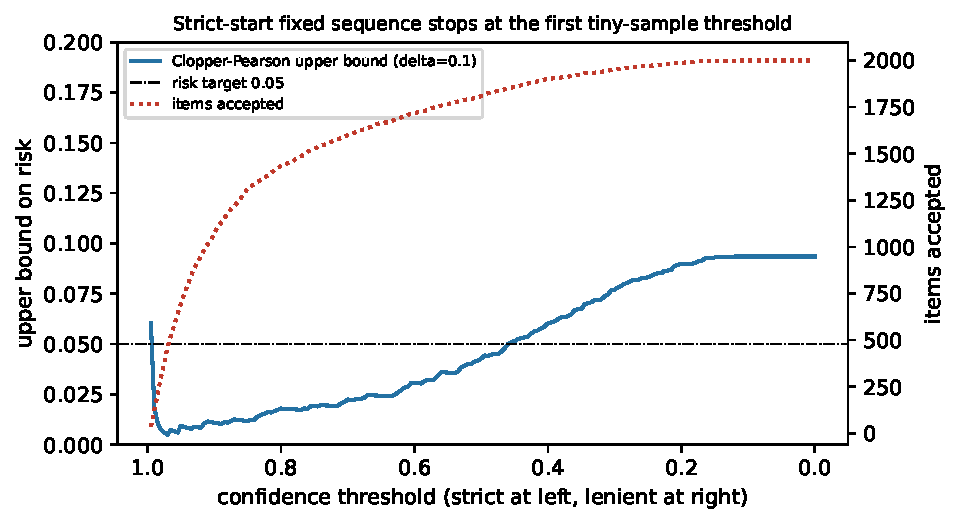
\includegraphics[width=0.7\textwidth]{fig4_strict_sequence_pitfall.pdf}
\caption{Why strict-start fixed-sequence selection almost never deploys: the first non-empty
thresholds accept too few items for the upper bound to fall below the target.}\end{figure}

\subsection{Teacher noise}
We labelled 2{,}000 random messages per task with Claude Haiku 5.5 using a schema-constrained
prompt (total spend about USD 0.9) and built two students per split: one distilled from the
teacher's labels and one trained on gold labels outside the labelled sample. Pools have 1{,}000
items; gates are fitted on calibration draws of teacher disagreement and evaluated against either
teacher disagreement or gold error (Table~\ref{tab:exp1b}).

\begin{table}[t]\centering\footnotesize
\begin{tabular}{llrrrrr}
\toprule
Task / student & $\alpha$ & method & deploy & viol.\ (teacher) & viol.\ (gold) & cov.\\
\midrule
B77 distilled & 0.10 & naive & 1.00 & 0.462 & 1.000 & 0.72\\
B77 distilled & 0.10 & wilson & 1.00 & 0.045 & 0.987 & 0.64\\
B77 distilled & 0.10 & bonferroni & 1.00 & 0.000 & 0.697 & 0.52\\
B77 distilled & 0.10 & holm & 1.00 & 0.001 & 0.728 & 0.53\\
B77 gold-trained & 0.10 & naive & 1.00 & 0.475 & 0.000 & 0.52\\
B77 gold-trained & 0.10 & wilson & 0.96 & 0.038 & 0.000 & 0.31\\
B77 gold-trained & 0.10 & bonferroni & 0.10 & 0.000 & 0.000 & 0.03\\
B77 gold-trained & 0.10 & holm & 0.10 & 0.000 & 0.000 & 0.03\\
CL150 distilled & 0.10 & naive & 1.00 & 0.484 & 0.844 & 0.79\\
CL150 distilled & 0.10 & wilson & 1.00 & 0.036 & 0.273 & 0.67\\
CL150 distilled & 0.10 & bonferroni & 0.96 & 0.000 & 0.003 & 0.46\\
CL150 distilled & 0.10 & holm & 0.96 & 0.001 & 0.008 & 0.48\\
CL150 gold-trained & 0.10 & naive & 1.00 & 0.302 & 0.000 & 0.99\\
CL150 gold-trained & 0.10 & wilson & 1.00 & 0.020 & 0.000 & 0.93\\
CL150 gold-trained & 0.10 & bonferroni & 0.70 & 0.000 & 0.000 & 0.55\\
CL150 gold-trained & 0.10 & holm & 0.70 & 0.000 & 0.000 & 0.56\\
\bottomrule
\end{tabular}

\caption{Violation rate (share of calibration draws whose chosen threshold has true risk above
$\alpha=0.10$) against the teacher and against gold, $m=400$, three splits (generated from
\texttt{results/exp1b\_*}).}\label{tab:exp1b}\end{table}

\subsection{Drift and audit sampling}
We built pre- and post-shift pools from real embeddings: a class-prior shift, word-level
perturbation, and unseen classes. A uniformly random fraction of decisions is audited; policies are a
static Holm gate, a rolling naive gate and a rolling Holm gate on the last 1{,}000 audited labels
(Table~\ref{tab:exp2}). Each recalibration carries its own $\delta$; the guarantee over repeated
recalibrations is not family-wise controlled.

\begin{table}[t]\centering\footnotesize
\begin{tabular}{llrrrr}
\toprule
Shift (Banking77) & policy & audit & post risk & post cov. & blocks $>\alpha$\\
\midrule
prior & static\_holm & 0.10 & 0.055 & 0.87 & 0.65\\
prior & rolling\_naive & 0.10 & 0.064 & 0.89 & 0.82\\
prior & rolling\_holm & 0.10 & 0.040 & 0.81 & 0.21\\
perturbed & static\_holm & 0.10 & 0.047 & 0.79 & 0.39\\
perturbed & rolling\_naive & 0.10 & 0.059 & 0.83 & 0.73\\
perturbed & rolling\_holm & 0.10 & 0.035 & 0.75 & 0.12\\
unseen & static\_holm & 0.10 & 0.359 & 0.70 & 1.00\\
unseen & rolling\_naive & 0.10 & 0.221 & 0.49 & 0.99\\
unseen & rolling\_holm & 0.10 & 0.158 & 0.29 & 0.83\\
\bottomrule
\end{tabular}

\caption{Banking77 drift streams, 10\% audit rate, 100 streams per cell, $\alpha=0.05$; ``blocks
$>\alpha$'' is the share of 500-decision post-shift blocks whose accepted-risk exceeds $\alpha$
(generated from \texttt{results/exp2\_*}).}\label{tab:exp2}\end{table}

\section{Limitations}
One teacher model and one prompt; teacher agreement with gold labels is measured on 2{,}000 items
per task and the benchmark gold labels have their own errors. One frozen encoder and one student
family. Finite-population evaluation on pools of 1{,}000 items; calibration sizes up to 400 in the
teacher-noise study. Drift shifts are constructions on real data, one instance each, single student
seed; the drift monitor assumes a constant mean and is used only as a change alarm. Repeated
recalibration is not family-wise controlled. Comparison with TRACER's certification is by reading
its code and changelog, not by running it. No claim of novelty is made for the cascade idea or for
conformal-style certification; a systematic literature check is still outstanding.

\section{Conclusion}
On these tasks, choosing a threshold on the sample that is supposed to validate it fails about half
the time near the achievable risk, valid selection is affordable, a certified agreement target does
not certify correctness when the reference is imperfect, and adapting to drift is limited by the
audit-label budget. These are preliminary findings from a small study.

\bibliographystyle{plainnat}
\bibliography{references}
\end{document}
